\documentclass[11pt,letterpaper]{article}

\usepackage[T1]{fontenc}
\usepackage[utf8]{inputenc}
\usepackage{lmodern}
\usepackage[letterpaper,margin=1in]{geometry}
\usepackage{microtype}
\usepackage{amsmath,amssymb}
\usepackage{booktabs,tabularx,array}
\usepackage[font=small,labelfont=bf,labelsep=period]{caption}
\usepackage{enumitem}
\usepackage{tikz}
\usetikzlibrary{positioning,arrows.meta}
\usepackage{xcolor}
\usepackage{xurl}
\usepackage[
  colorlinks=true,
  linkcolor=blue,
  citecolor=blue,
  urlcolor=blue
]{hyperref}
\urlstyle{same}

\hypersetup{
  pdftitle={A Factor-of-Ten Inconsistency in a Cited Cold-Seep Area and Its Conditional Effect on a Published Global Fe-OC Stock Endpoint},
  pdfauthor={UCP Technology LLC},
  pdfsubject={A provenance audit and conditional arithmetic reanalysis},
  pdfkeywords={cold seeps, iron-bound organic carbon, global stock, numerical provenance, citation-chain transmission}
}

\pagestyle{plain}
\setcounter{secnumdepth}{2}
\setcounter{tocdepth}{2}
\newcolumntype{Y}{>{\raggedright\arraybackslash}X}
\newcolumntype{L}[1]{>{\raggedright\arraybackslash}p{#1}}

\title{\bfseries A Factor-of-Ten Inconsistency in a Cited Cold-Seep Area and Its Conditional Effect on a Published Global Fe-OC Stock Endpoint}
\author{UCP Technology LLC\\[3pt]
  \small\href{https://ucptechnology.ai}{ucptechnology.ai}}
\date{\small Version: August 30, 2026}

\begin{document}
\maketitle

\begin{abstract}
Ye et al.\ (2026) report 142--218 Tg C of iron-bound organic carbon (Fe-OC) in the upper 30 cm of mature cold-seep sediments after applying a published global seep-area interval of $2.05$--$3.15\times10^5$ km$^2$. We audited the numerical provenance of that interval and recalculated the corresponding lower endpoint from the public source record. Boetius and Wenzh\"ofer (2013) print a continental-slope area of 41 million km$^2$ and assume that active seep systems occupy approximately 0.05\% of it. Those nominal premises multiply to 20,500 km$^2$, or $2.05\times10^4$ km$^2$. Jiang et al.\ (2025) instead report $2.05\times10^5$ km$^2$ as the lower endpoint of a jointly cited range without an endpoint-specific derivation. Li et al.\ (2024) provide a separate nominal construction matching Jiang et al.'s reported upper endpoint, but not the lower one. The publication record therefore demonstrates an incompatibility between the reported lower endpoint and the identifiable cited premises; it is consistent with, but does not independently prove, factor-of-ten transmission from those premises. Ye et al.\ subsequently use the same published area value in an area-linear stock calculation. Substituting the nominal $2.05\times10^4$ km$^2$ value while leaving all other terms unchanged changes the corresponding endpoint from approximately 142 to approximately 14.2 Tg C. A row-weighted calculation from the public source rows also yields 0.14\%, numerically matching the reported Fe-OC input; the public files do not disclose the aggregation rule. The result is a conditional arithmetic substitution to a published endpoint, not an estimate of the true global cold-seep area or Fe-OC stock.
\end{abstract}

\noindent\textbf{Keywords.}
cold seeps; iron-bound organic carbon; global stock; numerical provenance;
citation-chain transmission; conditional reanalysis.

\clearpage
\tableofcontents

\section{Introduction}

Global stock calculations commonly combine a locally measured concentration with a spatial domain over which that concentration is upscaled. In an area-linear calculation, the provenance of the area term is therefore as consequential as the measured concentration. This paper concerns correction scholarship: it audits one published numerical chain and does not estimate the true global cold-seep area or global Fe-OC inventory.

Ye et al.\ measured Fe-OC across stages of marine cold-seep development and estimated a mature-seep global stock~\cite{ye2026}. In Section 4.3 of their article, they apply an estimated global seep area of $2.05$--$3.15\times10^5$ km$^2$ to the average Fe-OC content in the upper 0--30 cm of mature-seep sediments. They cite Jiang et al.\ and Li et al.\ for the area and report approximately 142--218 Tg C~\cite{jiang2025,li2024}.

Jiang et al.\ had reported the same $2.05$--$3.15\times10^5$ km$^2$ interval while jointly citing Boetius and Wenzh\"ofer and Li et al.~\cite{jiang2025,boetius2013,li2024}. The lower endpoint warrants a direct arithmetic check because Boetius and Wenzh\"ofer print both a continental-slope area of 41 million km$^2$ and an assumed active-seep occupation of approximately 0.05\%~\cite{boetius2013}. Their nominal product is 20,500 km$^2$, not 205,000 km$^2$.

We ask one question: what follows for Ye et al.'s corresponding stock endpoint if the nominal $2.05\times10^4$ km$^2$ product is substituted for the published $2.05\times10^5$ km$^2$ lower endpoint and all other terms are held fixed? We reconstruct the public source chain, test possible arithmetic and definitional alternatives, recalculate the adjacent mature-seep concentration from the public data, and evaluate the one-variable substitution. We distinguish throughout among a demonstrated incompatibility, a strong numerical-provenance inference, and an unobserved causal drafting history.

\section{Materials and methods}

\subsection{Scope, sources, and evidence hierarchy}

The audit was limited to the numerical lineage used for the lower area in Ye et al.'s Fe-OC stock. Primary versions of record, publisher-hosted supporting information, and author-deposited source data were prioritized. Sources and linked version records were checked through August 30, 2026.

The immediate area premises were verified in Boetius and Wenzh\"ofer: 41 million km$^2$ on printed page 725 and approximately 0.05\% on printed page 731~\cite{boetius2013}. The first statement cites Levin and Sibuet~\cite{levin2012}; the occupation assumption has no adjacent citation marker. The reported interval and its jointly cited references were checked in Jiang et al.'s article, supporting information, Supplementary Data workbook, and Source Data workbook~\cite{jiang2025}. Li et al.'s construction was checked in its version of record~\cite{li2024}. Ye et al.'s area, stock endpoints, layer depth, and concentration were checked in the Wiley article and supporting information, while the source rows were obtained from the authors' public OSF data record~\cite{ye2026}.

We classified evidence into three levels:
\begin{enumerate}[label=(\roman*),leftmargin=2.1em]
\item \emph{demonstrated}: a number, citation, or use is present in the public source;
\item \emph{strongly inferred}: distinctive numbers and citation context identify a plausible endpoint source;
\item \emph{not demonstrated}: the private calculation direction, drafting step, or person that produced the exponent.
\end{enumerate}
Terms such as \emph{reported} and \emph{subsequently used} refer to publication-level evidence only.

\subsection{Nominal lower-area arithmetic and rescue tests}

Boetius and Wenzh\"ofer report that continental slopes cover approximately 41 million km$^2$ and assume that active seep systems occupy approximately 0.05\% of that area~\cite{boetius2013}. Converting the printed percentage gives
\begin{equation}
0.05\%=\frac{0.05}{100}=0.0005=5\times10^{-4}.
\label{eq:percent}
\end{equation}
The nominal product is
\begin{equation}
41{,}000{,}000\ \mathrm{km^2}\times0.0005
=20{,}500\ \mathrm{km^2}
=2.05\times10^4\ \mathrm{km^2}.
\label{eq:area}
\end{equation}

We tested the inverse conditions needed to produce 205,000 km$^2$. Holding 41 million km$^2$ fixed requires 0.5\%, holding 0.05\% fixed requires 410 million km$^2$, and otherwise an unreported factor of ten is required. The inspected articles, supplements, workbooks, repositories, and version records were searched for an alternative percentage, denominator, area-class conversion, active-to-total multiplier, unit conversion, or correction notice.

Jiang et al.\ also express their reported endpoints as approximately 0.057--0.087\% of global marine area~\cite{jiang2025}. We inverted those percentages to test whether they document an independent lower-end derivation. They imply denominators of approximately 359.65 and 362.07 million km$^2$, respectively. This is algebraically consistent with dividing the reported area endpoints by an approximately 360--362-million-km$^2$ marine domain. It does not document calculation direction or connect the 0.05\% continental-slope premise to 205,000 km$^2$.

\subsection{Heterogeneous endpoint constructions}

Jiang et al.\ print $2.05$--$3.15\times10^5$ km$^2$ and jointly cite Boetius and Wenzh\"ofer and Li et al., but provide neither an equation nor endpoint-specific citations~\cite{jiang2025}. Li et al.\ state that the active seep area at Haima is approximately 350 km$^2$ and that more than 900 cold seeps had been found globally~\cite{li2024}. Evaluating their extrapolation at a nominal count of 900 gives
\begin{equation}
350\ \mathrm{km^2}\times900
=315{,}000\ \mathrm{km^2}
=3.15\times10^5\ \mathrm{km^2}.
\label{eq:li}
\end{equation}
Because the area is approximate and the global count is stated as more than 900, this is a nominal numerical fingerprint matching Jiang et al.'s reported upper endpoint, not an empirical upper bound.

The two identifiable constructions are heterogeneous. They may differ in the spatial object called a seep or seep system, active patch versus broader field footprint, geographical completeness, clustering and overlap, and the representativeness of Haima. They are not confidence limits generated by one method. Table~\ref{tab:area-constructions} records the comparison used in this audit.

\begin{table}[tbp]
\caption{Heterogeneous nominal constructions associated with Jiang et al.'s reported area endpoints.}
\label{tab:area-constructions}
\centering
\small
\begin{tabularx}{\textwidth}{@{}L{0.18\textwidth}L{0.27\textwidth}L{0.20\textwidth}Y@{}}
\toprule
Construction & Spatial object and stage & Nominal rule & Evidentiary status \\
\midrule
Boetius--Wenzh\"ofer nominal product &
Continental-slope area occupied by active seep systems &
41 million km$^2$ times approximately 0.05\% &
Identifiable lower-end premises; not a validated lower confidence bound \\
\addlinespace
Li-aligned nominal product &
Haima active-seep area extrapolated across a nominal global seep count; representativeness assumed &
Approximately 350 km$^2$ times nominal 900 &
Fingerprint matching Jiang et al.'s reported upper endpoint; not an empirical upper bound \\
\bottomrule
\end{tabularx}
\end{table}

\subsection{Recalculation and weighting sensitivity of the Fe-OC input}

Ye et al.\ report mature-seep Fe-OC content of $0.14\pm0.06\%$ immediately before their stock calculation~\cite{ye2026}. The public source file contains two relevant blocks. The current-study block has 14 depth-interval rows: seven depths from each of two station profiles. Station labels differ between the official supporting table and the OSF source file, but the values and two-profile structure coincide. The historical block has eight mature-seep rows, all attributed to Hu et al.~\cite{hu2025}: one PC01-20 row and seven ROV5 depth-coded rows.

For each block and their pooled 22 rows, we calculated the arithmetic mean and sample standard deviation,
\begin{equation}
\bar{x}=\frac{1}{n}\sum_{i=1}^{n}x_i,
\qquad
s=\left(\frac{\sum_{i=1}^{n}(x_i-\bar{x})^2}{n-1}\right)^{1/2}.
\label{eq:mean-sd}
\end{equation}
These are depth-interval rows, not 22 independent studies or globally representative sites. The pooled calculation was retained only to calculate a row-weighted arithmetic mean and compare it numerically with the value printed by Ye et al.\ The public files do not disclose the authors' aggregation rule.

As a descriptive weighting sensitivity, we also gave equal weight to the current-study block mean and the Hu et al.\ block mean. A formal site-equal analysis was not performed because Table S7 does not define independent sites, cores, or replicates. An operational parsing of PC01 and ROV5 identifiers was retained only in the machine-readable supplement and is not treated as a site-level estimate.

The source tables report Fe-OC content, $c$, as a percentage of sediment dry mass. This quantity is distinct from $f_{\mathrm{Fe\mbox{-}OC}}$, the percentage of total organic carbon associated with iron reported in a separate column by Ye et al.~\cite{ye2026}. Only the dry-sediment Fe-OC mass percentage is used here.

\subsection{Primary one-variable endpoint substitution}

Ye et al.'s description applies the same concentration and 0--30 cm layer to the endpoints of one reported area interval~\cite{ye2026}. Under that fixed area-linear mapping, replacing only the lower area gives
\begin{equation}
M_{\mathrm{cf}}
=M_{\mathrm{published}}
\frac{A_{\mathrm{nominal}}}{A_{\mathrm{reported}}}
=142\ \mathrm{Tg\ C}\times\frac{20{,}500}{205{,}000}
=14.2\ \mathrm{Tg\ C}.
\label{eq:primary}
\end{equation}
This proportional substitution is the principal result. It does not require the undisclosed physical decomposition of the non-area terms.

\subsection{Secondary consistency checks}

First, we represented the reported area-linear calculation as
\begin{equation}
M=kA,
\label{eq:linear}
\end{equation}
where $k$ contains all non-area terms. If 205,000 and 315,000 km$^2$ were the actual computational inputs, both endpoints used one common $k$, no endpoint-specific concentration, thickness, or mass term was used, and 142 and 218 Tg C were rounded conventionally to the nearest whole Tg, then
\begin{equation}
141.5\le205{,}000k<142.5,
\qquad
217.5\le315{,}000k<218.5.
\label{eq:rounding}
\end{equation}
Intersecting these conditions and evaluating $20,500k$ gives a nominal endpoint-rounding consistency interval. It is not a scientific uncertainty interval.

Second, for an area $A$ in km$^2$, layer thickness $z$ in m, endpoint-compatible effective sediment-mass coefficient $\rho_{\mathrm{eff}}$ in g cm$^{-3}$, and Fe-OC content $c$ in percent of sediment dry mass, the dimensional identity is
\begin{equation}
M_{\mathrm{Tg}}
=A(10^6)z\rho_{\mathrm{eff}}(10^6)\frac{c}{100}(10^{-12})
=Az\rho_{\mathrm{eff}}\frac{c}{100}.
\label{eq:dimensional}
\end{equation}
Ye et al.\ disclose $A$, $z=0.30$ m, and $c=0.14\%$, but not the stock equation or sediment-mass coefficient. We therefore use $\rho_{\mathrm{eff}}=1.65$ g cm$^{-3}$ only as a reverse-engineered, nonunique, endpoint-compatible coefficient. It is not attributed to Ye et al.\ and is unnecessary to Equation~\eqref{eq:primary}.

\section{Results}

\subsection{The printed nominal premises give the factor-of-ten result}

Equation~\eqref{eq:area} is the direct product of the two values printed by Boetius and Wenzh\"ofer. Jiang et al.'s reported lower endpoint, $2.05\times10^5$ km$^2$, is exactly ten times that nominal product. None of the tested alternatives generated $2.05\times10^5$ km$^2$ from the printed 41-million-km$^2$ and 0.05\% premises.

The required 0.5\% occupation fraction is not printed by Boetius and Wenzh\"ofer. The required 410-million-km$^2$ denominator is not their continental-slope area and exceeds the approximately 360--362-million-km$^2$ marine domain implied by Jiang et al.'s accompanying percentages. No additional factor of ten or physical-area unit conversion was located. Because both source premises are approximate, 20,500 km$^2$ is a nominal product rather than four-significant-digit ecological knowledge; approximation cannot reconcile a full order-of-magnitude difference while both printed operands are retained.

\subsection{The publication record supports an incompatibility and a qualified transmission inference}

The lower mantissa 2.05 matches Equation~\eqref{eq:area}, while Jiang et al.'s exponent is one power of ten larger. Within the same jointly cited pair, Equation~\eqref{eq:li} matches the reported $3.15\times10^5$ km$^2$ upper endpoint. No other endpoint derivation was found in Jiang et al.'s article, supporting information, Supplementary Data, or Source Data.

These facts demonstrate that the reported lower endpoint is incompatible with the identifiable lower-end premises in the cited pair. The mantissa, exponent, joint citation, and negative search are consistent with factor-of-ten transmission, but the public record does not prove calculation direction, an exact drafting step, or individual responsibility. Jiang et al.'s 0.057--0.087\% statement is algebraically compatible with their reported endpoints but does not provide an independently documented derivation.

Ye et al.\ separately cite Boetius and Wenzh\"ofer for the statement that cold seeps cover less than 0.05\% of slope area~\cite{ye2026,boetius2013}. Later, they use the $2.05$--$3.15\times10^5$ km$^2$ interval cited to Jiang et al.\ and Li et al. Their article therefore establishes subsequent use of the same published value, not the origin of its exponent.

\begin{figure}[tbp]
\centering
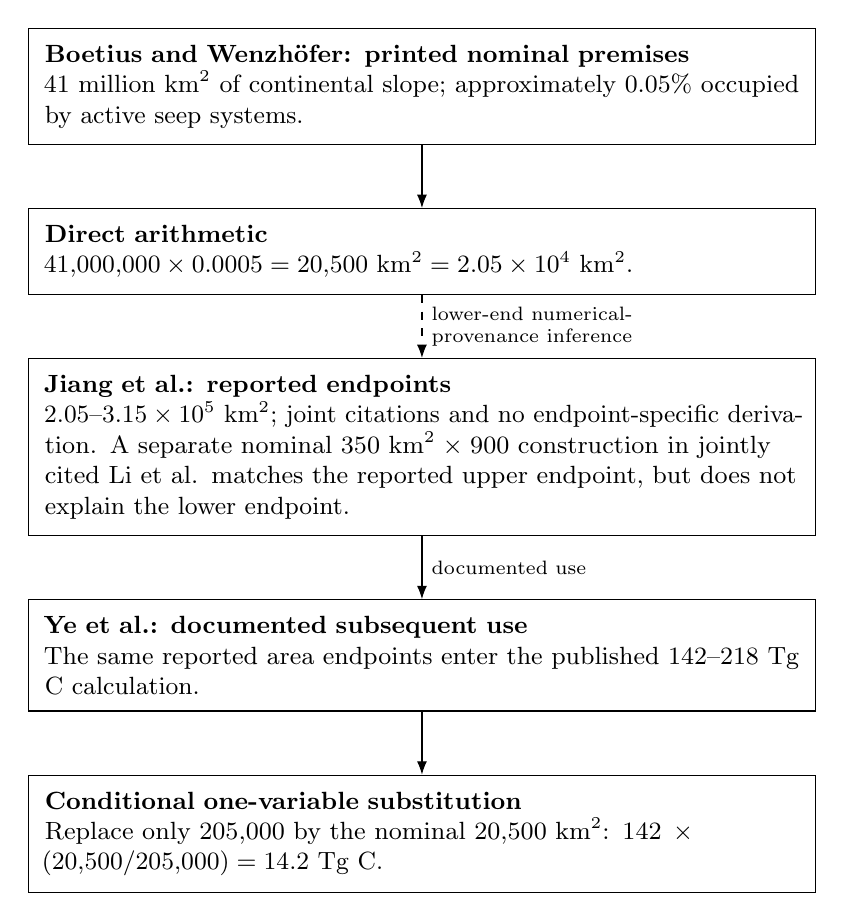
\begin{tikzpicture}[
  >=Latex,
  node distance=8mm,
  box/.style={draw, align=left, inner sep=6pt, text width=0.79\textwidth, font=\small}
]
\node[box] (bw) {\textbf{Boetius and Wenzh\"ofer: printed nominal premises}\\
41 million km$^2$ of continental slope; approximately 0.05\% occupied by active seep systems.};
\node[box, below=of bw] (arith) {\textbf{Direct arithmetic}\\
$41{,}000{,}000\times0.0005=20{,}500$ km$^2=2.05\times10^4$ km$^2$.};
\node[box, below=of arith] (jiang) {\textbf{Jiang et al.: reported endpoints}\\
$2.05$--$3.15\times10^5$ km$^2$; joint citations and no endpoint-specific derivation. A separate nominal $350$ km$^2\times900$ construction in jointly cited Li et al. matches the reported upper endpoint, but does not explain the lower endpoint.};
\node[box, below=of jiang] (ye) {\textbf{Ye et al.: documented subsequent use}\\
The same reported area endpoints enter the published 142--218 Tg C calculation.};
\node[box, below=of ye] (cf) {\textbf{Conditional one-variable substitution}\\
Replace only 205,000 by the nominal 20,500 km$^2$: $142\times(20{,}500/205{,}000)=14.2$ Tg C.};

\draw[->] (bw) -- (arith);
\draw[dashed,->] (arith) -- node[right,font=\scriptsize,align=left]{lower-end numerical-\\provenance inference} (jiang);
\draw[->] (jiang) -- node[right,font=\scriptsize]{documented use} (ye);
\draw[->] (ye) -- (cf);
\end{tikzpicture}
\caption{Publication-level numerical chain. Solid arrows denote direct arithmetic, documented subsequent use, or the stated conditional operation. The dashed arrow marks the lower-end source inference from the distinctive numerical fingerprint; it does not claim access to private drafting history. The final value is a conditional area substitution, not a global-stock estimate.}
\label{fig:chain}
\end{figure}

\subsection{The public rows yield a row-weighted match to the reported Fe-OC input}

The 14 current-study depth rows sum to 1.52\%, with mean 0.108571\% and row sample SD 0.024133\%. The eight Hu et al.\ rows sum to 1.56\%, with mean 0.195000\% and row sample SD 0.055806\%. The historical block mean is approximately 80\% higher than the current-study block mean.

Pooling all 22 depth-interval rows gives mean 0.140000\% and row sample SD 0.056653\%, which round to the $0.14\pm0.06\%$ printed by Ye et al. This row-weighted arithmetic calculation numerically reproduces the reported value; the public files do not establish that it was the authors' aggregation rule. The $\pm0.06\%$ value is a sample SD across rows, not a standard error, confidence interval, between-site uncertainty, or propagated stock uncertainty.

Equal weighting of the two source-study means gives 0.151786\%, 8.42\% above the row-pooled value. Table~\ref{tab:concentration} reports this as a descriptive sensitivity, not a replacement global concentration. Analytical comparability, row independence, and global representativeness are not established. Under any fixed concentration and other area-linear terms, however, replacing 205,000 by 20,500 km$^2$ still divides the corresponding stock endpoint by exactly ten.

\begin{table}[tbp]
\caption{Source-row structure and descriptive weighting sensitivity for mature-seep Fe-OC content.}
\label{tab:concentration}
\centering
\small
\begin{tabularx}{\textwidth}{@{}L{0.25\textwidth}L{0.24\textwidth}L{0.18\textwidth}Y@{}}
\toprule
Calculation & Source structure & Mean Fe-OC (\%) & Interpretation \\
\midrule
Current-study block &
14 depth rows; two station profiles, seven depths each &
0.108571 &
Row SD 0.024133\% \\
\addlinespace
Hu et al.\ historical block &
Eight rows; one PC01-20 row and seven ROV5 depth-coded rows &
0.195000 &
Row SD 0.055806\% \\
\addlinespace
Row-weighted pooling &
All 22 depth rows &
0.140000 &
Row SD 0.056653\%; numerically matches the reported $0.14\pm0.06\%$ \\
\addlinespace
Source-study-equal sensitivity &
Equal weight to the two block means &
0.151786 &
Descriptive weighting check; not a meta-analysis \\
\bottomrule
\end{tabularx}
\end{table}

\subsection{The one-variable substitution changes the corresponding endpoint to approximately 14.2 Tg C}

Equation~\eqref{eq:primary} gives the central numerical consequence directly:
\[
142\ \mathrm{Tg\ C}\times\frac{20{,}500}{205{,}000}
=14.2\ \mathrm{Tg\ C}.
\]
If Jiang et al.'s reported upper endpoint is retained unchanged, the two displayed stock endpoints would become a heterogeneous, model-conditioned span of approximately 14.2--218 Tg C. That span is not a confidence interval or uncertainty interval and has no statistical coverage interpretation.

The two printed stock-to-area ratios are
\[
\frac{142}{205{,}000}=0.000692683,
\qquad
\frac{218}{315{,}000}=0.000692063
\quad\mathrm{Tg\ C\ km^{-2}}.
\]
They differ by approximately 0.09\% relative to their mean, which is compatible with one common area-linear coefficient followed by whole-Tg reporting.

Under all four assumptions stated before Equation~\eqref{eq:rounding}, the common coefficient satisfies
\[
0.000690476\le k<0.000693651
\quad\mathrm{Tg\ C\ km^{-2}},
\]
and the substituted endpoint satisfies
\begin{equation}
14.15\le M_{\mathrm{cf}}<14.22\ \mathrm{Tg\ C}.
\label{eq:rounding-result}
\end{equation}
This is a nominal endpoint-rounding consistency interval. Its narrow width reflects compatibility with two rounded display values only; it does not represent ecological, sampling, area, sediment-mass, or model uncertainty. Full-precision bounds are retained in the reproducibility record.

Finally, Equation~\eqref{eq:dimensional} with $z=0.30$ m, $c=0.14\%$, and the endpoint-compatible $\rho_{\mathrm{eff}}=1.65$ g cm$^{-3}$ gives
\[
205{,}000\times0.30\times1.65\times\frac{0.14}{100}
=142.065\ \mathrm{Tg\ C},
\]
\[
315{,}000\times0.30\times1.65\times\frac{0.14}{100}
=218.295\ \mathrm{Tg\ C},
\]
and
\[
20{,}500\times0.30\times1.65\times\frac{0.14}{100}
=14.2065\ \mathrm{Tg\ C}.
\]
This secondary check shows dimensional compatibility with the displayed endpoints. It does not recover an author-reported coefficient or validate its physical interpretation.

\section{Discussion}

\subsection{Demonstrated arithmetic versus inferred causal history}

This analysis is a provenance correction, not a new global-area or stock estimate. The demonstrated result is simple: the two nominal values printed by Boetius and Wenzh\"ofer multiply to $2.05\times10^4$ km$^2$, while Jiang et al.\ report $2.05\times10^5$ km$^2$ without an endpoint-specific derivation. Ye et al.\ subsequently use that reported value in their area-linear stock calculation.

A causal account of how the exponent entered the literature is a stronger proposition. The matching mantissa, one-power exponent shift, joint citation, and absence of another public derivation are consistent with factor-of-ten transmission from the identifiable lower-end premises. They do not exclude an undocumented source, private calculation, or drafting transformation. Accordingly, the manuscript does not say that Ye et al.\ created the inconsistency or that a named Jiang et al.\ author performed an incorrect multiplication.

\subsection{What the 14.2 Tg C endpoint means}

Approximately 14.2 Tg C is the result of one controlled substitution in the published area-linear mapping. It is not a validated lower bound on the true global mature-seep Fe-OC stock. That stronger interpretation would require, among other things, a defensible global seep-area model, a globally representative concentration, a disclosed sediment-mass coefficient, a uniform or otherwise modeled depth, and commensurability between the area and observation domains.

The last condition is unresolved in the present record. Boetius and Wenzh\"ofer's area premise concerns \emph{active seep systems}, whereas Ye et al.'s concentration is assigned to a \emph{mature} developmental stage. Their spatial and developmental categories have not been shown to be commensurate. The endpoint substitution therefore corrects an arithmetic input under the inherited calculation but does not repair the conceptual basis of the global upscaling.

Likewise, the two area endpoints are heterogeneous nominal constructions rather than statistical bounds. Li et al.'s wording \emph{more than 900} does not generate an empirical upper bound at 900, and the representativeness of the Haima area is outside this audit. Retaining 218 Tg C only holds the reported upper endpoint fixed; it does not validate it.

\subsection{Why the unresolved gaps do not rescue the arithmetic}

Boetius and Wenzh\"ofer cite Levin and Sibuet for the 41-million-km$^2$ continental-slope statement~\cite{boetius2013,levin2012}. The exact sentence-level route remains unresolved. Menot et al.\ report an approximately 40-million-km$^2$ deep-margin domain and corroborate the scale, but cannot be assigned as the exact source~\cite{menot2010}. This bibliographic gap does not alter the product of the two values Boetius and Wenzh\"ofer themselves print. A 205,000-km$^2$ result at 0.05\% requires 410 million km$^2$; at 41 million km$^2$, it requires 0.5\%.

Ye et al.\ do not disclose the exact stock equation or sediment-mass coefficient. This prevents a fully source-disclosed physical reconstruction and is why 1.65 g cm$^{-3}$ remains a nonunique effective coefficient. It cannot rescue the lower area because any otherwise fixed area-linear mapping changes by exactly the same factor as area. Equation~\eqref{eq:primary} therefore does not depend on knowing the physical decomposition of $k$.

\subsection{Corrective and prepublication value}

A transparent published correction could state the nominal product of the Boetius--Wenzh\"ofer premises, identify the heterogeneous sources associated with the two reported endpoints, and disclose the full Ye et al.\ stock equation and sediment-mass coefficient. These steps would make the numerical chain independently evaluable without changing Ye et al.'s underlying measurements.

The negative source search is necessarily bounded. Before publication, the reproducibility archive should be deposited in a persistent, versioned repository, and the corresponding authors of Jiang et al.\ and Ye et al.\ should be invited to clarify the endpoint derivation and stock coefficient. No author clarification had been obtained by the version date. A documented alternative source could change the provenance interpretation, but not Equation~\eqref{eq:area}.

\section{Limitations}

\begin{enumerate}[label=(\roman*),leftmargin=2.1em]
\item The ultimate Levin-to-Boetius ancestry of the 41-million-km$^2$ denominator remains unresolved. The analysis multiplies the premises printed by Boetius and Wenzh\"ofer and does not claim an original derivation.

\item Jiang et al.\ jointly cite Boetius and Wenzh\"ofer and Li et al.\ without assigning individual endpoints. The endpoint-source mapping is a strong numerical-provenance inference, not explicit citation syntax.

\item Jiang et al.'s marine-area percentages are algebraically compatible with their reported endpoints, but the public record does not establish whether areas or percentages were calculated first.

\item Ye et al.\ do not publish their exact stock equation or sediment-mass coefficient. The 1.65 g cm$^{-3}$ value is an endpoint-compatible, reverse-engineered coefficient and is not necessary to the primary proportional result.

\item The 22 Fe-OC rows are depth intervals, not independent global sites. The pooled SD is not between-site uncertainty. Analytical comparability and global representativeness are unestablished, and Table S7 does not support a formal site-equal analysis.

\item The active-seep-system area premise has not been shown to be commensurate with Ye et al.'s mature-seep observations. The one-variable result is consequently not an ecological lower bound.

\item The two area endpoints arise from heterogeneous nominal constructions. Neither the area pair nor the corresponding 14.2--218 Tg C display should be interpreted as a confidence or uncertainty interval.

\item The nominal endpoint-rounding consistency interval assumes exact computational use of the displayed areas, one common coefficient, no endpoint-specific non-area terms, and nearest-whole-Tg rounding. It measures display compatibility only.

\item The bounded negative search cannot exclude private sources or future corrections. The current supplement lacks a persistent public DOI, and no author clarification has yet been sought.
\end{enumerate}

\section{Conclusion}

The nominal values printed by Boetius and Wenzh\"ofer -- 41 million km$^2$ and approximately 0.05\% -- yield $2.05\times10^4$ km$^2$. Jiang et al.\ report $2.05\times10^5$ km$^2$ without an endpoint-specific derivation, and Ye et al.\ subsequently use that published value in an area-linear Fe-OC stock calculation. Substituting the nominal $2.05\times10^4$ km$^2$ value while leaving all other terms unchanged changes the corresponding published endpoint from approximately 142 to approximately 14.2 Tg C. The publication record demonstrates the numerical incompatibility and is consistent with factor-of-ten citation-chain transmission, but does not independently prove its private causal history. This is a conditional arithmetic substitution to a published endpoint, not an estimate of the true global cold-seep area or Fe-OC stock.

\section{Data and code availability}

Ye et al.'s underlying Fe-OC source data are publicly available at \url{https://osf.io/6ymra}~\cite{ye2026}. This repository includes \path{Reproducibility_Supplement.zip}, which contains the required extracted rows, executable calculations, machine-readable outputs, verification tests, and source-value record. Source locators, access dates, and checksums are documented in the repository. Third-party articles and supplemental files are linked rather than redistributed.

For journal submission, the supplement should be cited from a versioned repository with a persistent identifier. No new observational data were generated.

\begin{thebibliography}{99}
\small

\bibitem{boetius2013}
A. Boetius and F. Wenzh\"ofer,
Seafloor oxygen consumption fuelled by methane from cold seeps,
\emph{Nature Geoscience} \textbf{6} (2013), 725--734.
\href{https://doi.org/10.1038/ngeo1926}
{\nolinkurl{https://doi.org/10.1038/ngeo1926}}.

\bibitem{hu2025}
Y. Hu, K. Li, J. C. Faust, J. Peckmann, D. Zhang, L. Chen, Q. Liang,
D. Chen, and D. Feng,
Stability of reactive iron-bound organic carbon during sulfidization of iron oxides:
Insights from methane-seep sediments,
\emph{Geophysical Research Letters} \textbf{52} (2025), e2024GL112119.
\href{https://doi.org/10.1029/2024GL112119}
{\nolinkurl{https://doi.org/10.1029/2024GL112119}}.

\bibitem{jiang2025}
Q. Jiang, L. Cao, Y. Han, et al.,
Cold seeps are potential hotspots of deep-sea nitrogen loss driven by microorganisms across 21 phyla,
\emph{Nature Communications} \textbf{16} (2025), Article 1646.
\href{https://doi.org/10.1038/s41467-025-56774-1}
{\nolinkurl{https://doi.org/10.1038/s41467-025-56774-1}}.

\bibitem{levin2012}
L. A. Levin and M. Sibuet,
Understanding continental margin biodiversity: A new imperative,
\emph{Annual Review of Marine Science} \textbf{4} (2012), 79--112.
\href{https://doi.org/10.1146/annurev-marine-120709-142714}
{\nolinkurl{https://doi.org/10.1146/annurev-marine-120709-142714}}.

\bibitem{li2024}
J. Li, X. Dong, Y. Tang, et al.,
Deep sea cold seeps are a sink for mercury and source for methylmercury,
\emph{Communications Earth \& Environment} \textbf{5} (2024), Article 324.
\href{https://doi.org/10.1038/s43247-024-01484-7}
{\nolinkurl{https://doi.org/10.1038/s43247-024-01484-7}}.

\bibitem{menot2010}
L. Menot, M. Sibuet, R. S. Carney, et al.,
New perceptions of continental margin biodiversity,
in A. D. McIntyre (ed.), \emph{Life in the World's Oceans: Diversity,
Distribution and Abundance}, Wiley-Blackwell, 2010, pp. 79--102.
\href{https://doi.org/10.1002/9781444325508.ch5}
{\nolinkurl{https://doi.org/10.1002/9781444325508.ch5}}.

\bibitem{ye2026}
W. Ye, Y. Chen, C. Yang, et al.,
Dynamics of iron-bound organic carbon across different development stages of marine cold seeps,
\emph{Global Biogeochemical Cycles} \textbf{40} (2026), e2025GB008889.
\href{https://doi.org/10.1029/2025GB008889}
{\nolinkurl{https://doi.org/10.1029/2025GB008889}}.

\end{thebibliography}

\end{document}
